\documentclass{beamer}
\usetheme[sectionpage=none]{metropolis}

\usepackage{pgfpages}
%\setbeameroption{show notes on second screen=right}

\usepackage{isabelle,isabellesym}
\newcommand*{\term}[1]{{\isaspacing\isastyle \input{#1}}}
\newcommand*{\Term}[1]{{\isaspacing\isastyle #1}}
\newcommand*{\mTerm}[1]{\text{\Term{#1}}}

\usepackage{mathtools}

\DeclarePairedDelimiter\card{\lvert}{\rvert}
\newcommand{\cons}{\mathbin{\#}}

\usepackage{algorithm2e}
\resetcounteronoverlays{algocf}

\usepackage{tikz}
\usepackage{tkz-graph}
\usetikzlibrary{calc,shapes.multipart,chains,arrows,backgrounds}

\usepackage{adjustbox}

\SetKwInput{Init}{Initialization}
\SetKwInput{Online}{Online Matching}
\SetKwFor{Arrival}{On arrival of}{}{}
\SetKwIF{If}{ElseIf}{Else}{if}{}{else if}{else}{}

\title{Formal Verification of the RANKING algorithm for Online Bipartite Matching}
\author{Christoph Madlener}
\date{22.06.2022}

\begin{document}
\begin{frame}[plain]
  \titlepage
\end{frame}

\section{Introduction}
\begin{frame}
  \frametitle{Online Bipartite Matching (OBM)}
  \begin{columns}
    \begin{column}{.65\textwidth}
      \begin{exampleblock}{Input}
        \begin{itemize}[<+->]
          \item \emph{bipartite} graph $G = (U,V,E)$
          \item \emph{offline} vertices $V$ are known
          \item \emph{online} vertices $U$ reveal edges on arrival
        \end{itemize}
      \end{exampleblock}
    \end{column}
    \begin{column}{.3\textwidth}
      \vspace{0.5em}
      
      \only<1>{
        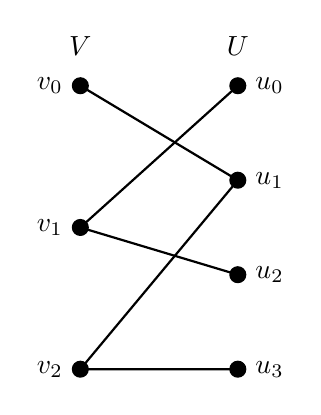
\begin{tikzpicture}
          \node at (0,1.5){$V$};
          \node at (2,1.5){$U$};
          \GraphInit[vstyle=Classic];
          \SetVertexNormal[MinSize=1pt,FillColor=black]
          \Vertices[Math,x=0,y=1,Lpos=180,dir=\SO,unit=1.8]{line}{v_0, v_1, v_2};
          \Vertices[Math,x=2,y=1,dir=\SO,unit=1.2]{line}{u_0,u_1,u_2,u_3};
          \Edge(v_0)(u_1);
          \Edge(v_1)(u_0);
          \Edge(v_1)(u_2);
          \Edge(v_2)(u_1);
          \Edge(v_2)(u_3);
        \end{tikzpicture} 
      }%
      \only<2>{
        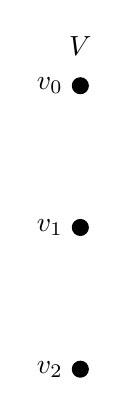
\begin{tikzpicture}
          \node at (0,1.5){$V$};
          \GraphInit[vstyle=Classic];
          \SetVertexNormal[MinSize=1pt,FillColor=black]
          \Vertices[Math,x=0,y=1,Lpos=180,dir=\SO,unit=1.8]{line}{v_0, v_1, v_2};
        \end{tikzpicture} 
      }%
      \only<3>{
        \begin{tikzpicture}
          \node at (0,1.5){$V$};
          \node at (2,1.5){$\pi$};
          \GraphInit[vstyle=Classic];
          \SetVertexNormal[MinSize=1pt,FillColor=black]
          \Vertices[Math,x=0,y=1,Lpos=180,dir=\SO,unit=1.8]{line}{v_0, v_1, v_2};
        \end{tikzpicture} 
      }%
      \only<4>{
        \begin{tikzpicture}
          \node at (0,1.5){$V$};
          \node at (2,1.5){$\pi$};
          \GraphInit[vstyle=Classic];
          \SetVertexNormal[MinSize=1pt,FillColor=black]
          \Vertices[Math,x=0,y=1,Lpos=180,dir=\SO,unit=1.8]{line}{v_0, v_1, v_2};
          \Vertices[Math,x=2,y=1,dir=\SO,unit=1.2]{line}{u_0};
          \Edge(v_1)(u_0);
        \end{tikzpicture} 
      }%
      \only<5>{
        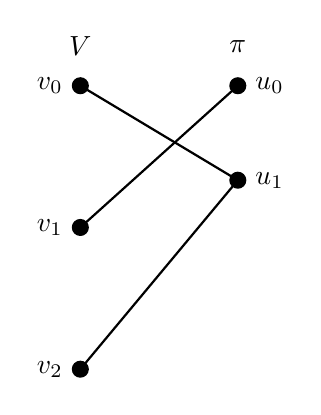
\begin{tikzpicture}
          \node at (0,1.5){$V$};
          \node at (2,1.5){$\pi$};
          \GraphInit[vstyle=Classic];
          \SetVertexNormal[MinSize=1pt,FillColor=black]
          \Vertices[Math,x=0,y=1,Lpos=180,dir=\SO,unit=1.8]{line}{v_0, v_1, v_2};
          \Vertices[Math,x=2,y=1,dir=\SO,unit=1.2]{line}{u_0,u_1};
          \Edge(v_1)(u_0);
          \Edge(v_0)(u_1);
          \Edge(v_2)(u_1);
        \end{tikzpicture}
      }%
      \only<6>{
        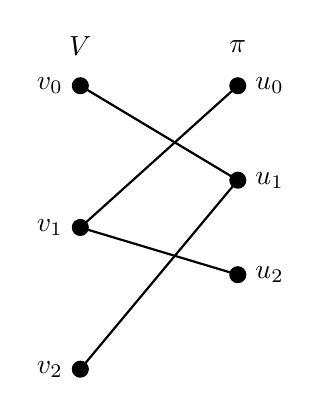
\begin{tikzpicture}
          \node at (0,1.5){$V$};
          \node at (2,1.5){$\pi$};
          \GraphInit[vstyle=Classic];
          \SetVertexNormal[MinSize=1pt,FillColor=black]
          \Vertices[Math,x=0,y=1,Lpos=180,dir=\SO,unit=1.8]{line}{v_0, v_1, v_2};
          \Vertices[Math,x=2,y=1,dir=\SO,unit=1.2]{line}{u_0,u_1,u_2};
          \Edge(v_1)(u_0);
          \Edge(v_0)(u_1);
          \Edge(v_2)(u_1);
          \Edge(v_1)(u_2);
        \end{tikzpicture}
      }%
      \only<7>{
        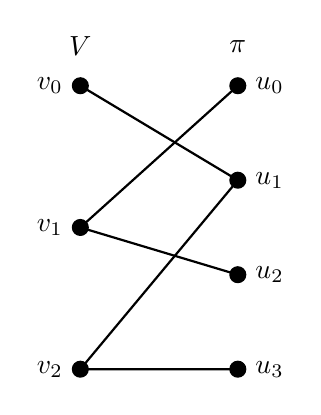
\begin{tikzpicture}
          \node at (0,1.5){$V$};
          \node at (2,1.5){$\pi$};
          \GraphInit[vstyle=Classic];
          \SetVertexNormal[MinSize=1pt,FillColor=black]
          \Vertices[Math,x=0,y=1,Lpos=180,dir=\SO,unit=1.8]{line}{v_0, v_1, v_2};
          \Vertices[Math,x=2,y=1,dir=\SO,unit=1.2]{line}{u_0,u_1,u_2,u_3};
          \Edge(v_1)(u_0);
          \Edge(v_0)(u_1);
          \Edge(v_2)(u_1);
          \Edge(v_1)(u_2);
          \Edge(v_2)(u_3);
        \end{tikzpicture}
      }%
      \only<8-9>{
        \begin{tikzpicture}
          \node at (0,1.5){$V$};
          \node at (2,1.5){$\pi$};
          \GraphInit[vstyle=Classic];
          \SetVertexNormal[MinSize=1pt,FillColor=black]
          \Vertices[Math,x=0,y=1,Lpos=180,dir=\SO,unit=1.8]{line}{v_0, v_1, v_2};
          \Vertices[Math,x=2,y=1,dir=\SO,unit=1.2]{line}{u_0};
          \Edge(v_1)(u_0);
        \end{tikzpicture}}%
      \only<10>{
        \begin{tikzpicture}
          \node at (0,1.5){$V$};
          \node at (2,1.5){$\pi$};
          \GraphInit[vstyle=Classic];
          \SetVertexNormal[MinSize=1pt,FillColor=black]
          \Vertex[Math,x=0,y=1,Lpos=180]{v_0};
          \SetVertexNormal[MinSize=1pt,FillColor=orange]
          \Vertex[Math,x=0,y=-0.8,Lpos=180]{v_1};
          \SetVertexNormal[MinSize=1pt,FillColor=black]
          \Vertex[Math,x=0,y=-2.6,Lpos=180]{v_2};
          \SetVertexNormal[MinSize=1pt,FillColor=blue]
          \Vertex[Math,x=2,y=1]{u_0};
          \Edge(v_1)(u_0);
        \end{tikzpicture}}%
      \only<11>{
        \begin{tikzpicture}
          \node at (0,1.5){$V$};
          \node at (2,1.5){$\pi$};
          \GraphInit[vstyle=Classic];
          \SetVertexNormal[MinSize=1pt,FillColor=black]
          \Vertex[Math,x=0,y=1,Lpos=180]{v_0};
          \Vertex[Math,x=0,y=-2.6,Lpos=180]{v_2};
          
          \SetVertexNormal[MinSize=1pt,FillColor=green]
          \Vertex[Math,x=0,y=-0.8,Lpos=180]{v_1};
          \Vertex[Math,x=2,y=1]{u_0};
          
          % matching edges
          \tikzset{EdgeStyle/.append style = {green}};
          \Edge(v_1)(u_0);
        \end{tikzpicture}}%
      \only<12>{
        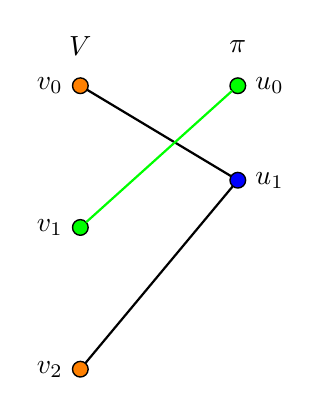
\begin{tikzpicture}
          \node at (0,1.5){$V$};
          \node at (2,1.5){$\pi$};
          \GraphInit[vstyle=Classic];
          \SetVertexNormal[MinSize=1pt,FillColor=black]
          
          \SetVertexNormal[MinSize=1pt,FillColor=orange]
          \Vertex[Math,x=0,y=1,Lpos=180]{v_0};
          \Vertex[Math,x=0,y=-2.6,Lpos=180]{v_2};
          
          \SetVertexNormal[MinSize=1pt,FillColor=blue]
          \Vertex[Math,x=2,y=-0.2]{u_1};
          
          \SetVertexNormal[MinSize=1pt,FillColor=green]
          \Vertex[Math,x=0,y=-0.8,Lpos=180]{v_1};
          \Vertex[Math,x=2,y=1]{u_0};
          
          \Edge(v_0)(u_1);
          \Edge(v_2)(u_1);
          
          % matching edges
          \tikzset{EdgeStyle/.append style = {green}};
          \Edge(v_1)(u_0);
        \end{tikzpicture}}%
      \only<13>{
        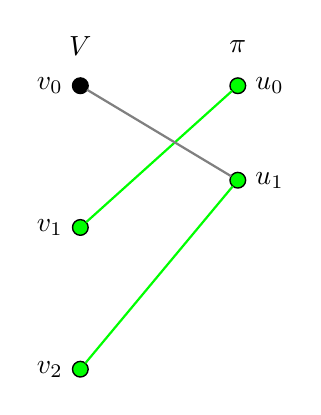
\begin{tikzpicture}
          \node at (0,1.5){$V$};
          \node at (2,1.5){$\pi$};
          \GraphInit[vstyle=Classic];
          \SetVertexNormal[MinSize=1pt,FillColor=black]
          \Vertex[Math,x=0,y=1,Lpos=180]{v_0};
          
          \SetVertexNormal[MinSize=1pt,FillColor=orange]
          
          \SetVertexNormal[MinSize=1pt,FillColor=blue]
          
          \SetVertexNormal[MinSize=1pt,FillColor=green]
          \Vertex[Math,x=0,y=-0.8,Lpos=180]{v_1};
          \Vertex[Math,x=0,y=-2.6,Lpos=180]{v_2};
          \Vertex[Math,x=2,y=1]{u_0};
          \Vertex[Math,x=2,y=-0.2]{u_1};
                    
          % matching edges
          \tikzset{EdgeStyle/.append style = {green}};
          \Edge(v_1)(u_0);
          \Edge(v_2)(u_1);
          
          % discarded eges
          \tikzset{EdgeStyle/.append style = {gray}};
          \Edge(v_0)(u_1);
        \end{tikzpicture}}%
      \only<14>{
        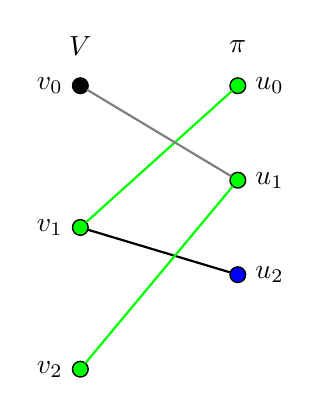
\begin{tikzpicture}
          \node at (0,1.5){$V$};
          \node at (2,1.5){$\pi$};
          \GraphInit[vstyle=Classic];
          \SetVertexNormal[MinSize=1pt,FillColor=black]
          \Vertex[Math,x=0,y=1,Lpos=180]{v_0};
          
          \SetVertexNormal[MinSize=1pt,FillColor=orange]
          
          \SetVertexNormal[MinSize=1pt,FillColor=blue]
          \Vertex[Math,x=2,y=-1.4]{u_2};
          
          \SetVertexNormal[MinSize=1pt,FillColor=green]
          \Vertex[Math,x=0,y=-0.8,Lpos=180]{v_1};
          \Vertex[Math,x=0,y=-2.6,Lpos=180]{v_2};
          \Vertex[Math,x=2,y=1]{u_0};
          \Vertex[Math,x=2,y=-0.2]{u_1};
          
          \Edge(v_1)(u_2);
                    
          % matching edges
          \tikzset{EdgeStyle/.append style = {green}};
          \Edge(v_1)(u_0);
          \Edge(v_2)(u_1);
          
          % discarded eges
          \tikzset{EdgeStyle/.append style = {gray}};
          \Edge(v_0)(u_1);
        \end{tikzpicture}}%
      \only<15>{
        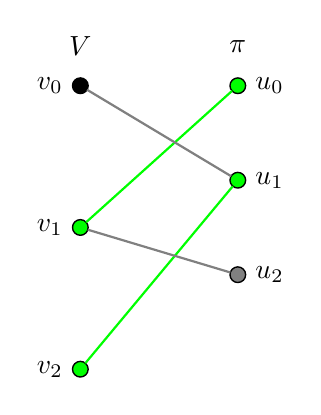
\begin{tikzpicture}
          \node at (0,1.5){$V$};
          \node at (2,1.5){$\pi$};
          \GraphInit[vstyle=Classic];
          \SetVertexNormal[MinSize=1pt,FillColor=black]
          \Vertex[Math,x=0,y=1,Lpos=180]{v_0};
          
          \SetVertexNormal[MinSize=1pt,FillColor=orange]
          
          \SetVertexNormal[MinSize=1pt,FillColor=blue]
          
          \SetVertexNormal[MinSize=1pt,FillColor=green]
          \Vertex[Math,x=0,y=-0.8,Lpos=180]{v_1};
          \Vertex[Math,x=0,y=-2.6,Lpos=180]{v_2};
          \Vertex[Math,x=2,y=1]{u_0};
          \Vertex[Math,x=2,y=-0.2]{u_1};
          
          \SetVertexNormal[MinSize=1pt,FillColor=gray]
          \Vertex[Math,x=2,y=-1.4]{u_2};
          
          % matching edges
          \tikzset{EdgeStyle/.append style = {green}};
          \Edge(v_1)(u_0);
          \Edge(v_2)(u_1);
          
          % discarded eges
          \tikzset{EdgeStyle/.append style = {gray}};
          \Edge(v_0)(u_1);
          \Edge(v_1)(u_2);
        \end{tikzpicture}}%
      \only<16>{
        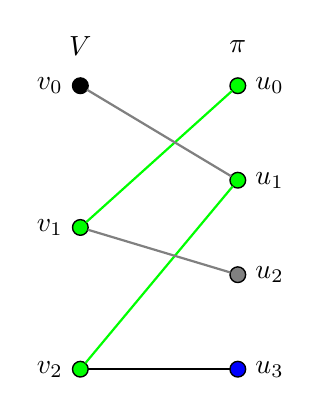
\begin{tikzpicture}
          \node at (0,1.5){$V$};
          \node at (2,1.5){$\pi$};
          \GraphInit[vstyle=Classic];
          \SetVertexNormal[MinSize=1pt,FillColor=black]
          \Vertex[Math,x=0,y=1,Lpos=180]{v_0};
          
          \SetVertexNormal[MinSize=1pt,FillColor=orange]
          
          \SetVertexNormal[MinSize=1pt,FillColor=blue]
          \Vertex[Math,x=2,y=-2.6]{u_3};
          
          \SetVertexNormal[MinSize=1pt,FillColor=green]
          \Vertex[Math,x=0,y=-0.8,Lpos=180]{v_1};
          \Vertex[Math,x=0,y=-2.6,Lpos=180]{v_2};
          \Vertex[Math,x=2,y=1]{u_0};
          \Vertex[Math,x=2,y=-0.2]{u_1};
          
          \SetVertexNormal[MinSize=1pt,FillColor=gray]
          \Vertex[Math,x=2,y=-1.4]{u_2};
          
          \Edge(v_2)(u_3);
          
          % matching edges
          \tikzset{EdgeStyle/.append style = {green}};
          \Edge(v_1)(u_0);
          \Edge(v_2)(u_1);
          
          % discarded eges
          \tikzset{EdgeStyle/.append style = {gray}};
          \Edge(v_0)(u_1);
          \Edge(v_1)(u_2);
        \end{tikzpicture}}%
      \only<17>{
        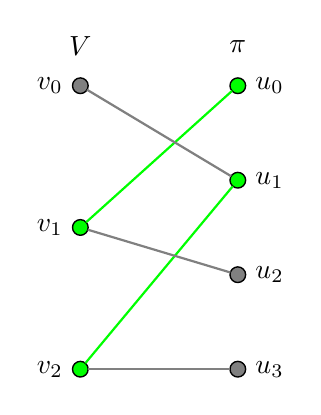
\begin{tikzpicture}
          \node at (0,1.5){$V$};
          \node at (2,1.5){$\pi$};
          \GraphInit[vstyle=Classic];
          \SetVertexNormal[MinSize=1pt,FillColor=black]
          
          \SetVertexNormal[MinSize=1pt,FillColor=orange]
          
          \SetVertexNormal[MinSize=1pt,FillColor=blue]
          
          \SetVertexNormal[MinSize=1pt,FillColor=green]
          \Vertex[Math,x=0,y=-0.8,Lpos=180]{v_1};
          \Vertex[Math,x=0,y=-2.6,Lpos=180]{v_2};
          \Vertex[Math,x=2,y=1]{u_0};
          \Vertex[Math,x=2,y=-0.2]{u_1};
          
          \SetVertexNormal[MinSize=1pt,FillColor=gray]
          \Vertex[Math,x=0,y=1,Lpos=180]{v_0};
          \Vertex[Math,x=2,y=-1.4]{u_2};
          \Vertex[Math,x=2,y=-2.6]{u_3};
          
          % matching edges
          \tikzset{EdgeStyle/.append style = {green}};
          \Edge(v_1)(u_0);
          \Edge(v_2)(u_1);
          
          % discarded eges
          \tikzset{EdgeStyle/.append style = {gray}};
          \Edge(v_0)(u_1);
          \Edge(v_1)(u_2);
          \Edge(v_2)(u_3);
        \end{tikzpicture}
      }%
    \end{column}
  \end{columns}
  \onslide<8->
  \begin{alertblock}{Task}
    \begin{itemize}
      \item<8-> match as many vertices as possible
      \item<9-> on arrival of $u \in U$, \alert{irrevocably} match to \emph{unmatched}
        neighbor $v \in V$ (or not)
    \end{itemize}   
  \end{alertblock}
\end{frame}

\begin{frame}
  \frametitle{Competitive Ratio}
  \begin{columns}
    \begin{column}{.65\textwidth}
      \begin{alertblock}{Performance of online algorithm $\mathcal{A}$}
        \begin{itemize}
          \item Compare $\mathcal{A}$ to best offline algorithm
        \end{itemize}
      \end{alertblock}
    \end{column}
    \begin{column}{.3\textwidth}
      \only<1>{
        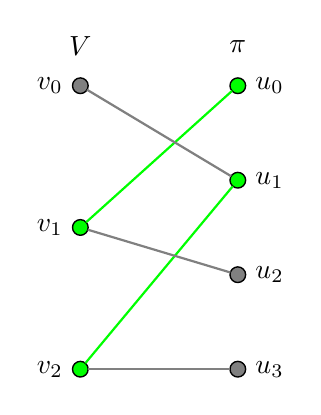
\begin{tikzpicture}
          \node at (0,1.5){$V$};
          \node at (2,1.5){$\pi$};
          \GraphInit[vstyle=Classic];
          \SetVertexNormal[MinSize=1pt,FillColor=black]
          
          \SetVertexNormal[MinSize=1pt,FillColor=orange]
          
          \SetVertexNormal[MinSize=1pt,FillColor=blue]
          
          \SetVertexNormal[MinSize=1pt,FillColor=green]
          \Vertex[Math,x=0,y=-0.8,Lpos=180]{v_1};
          \Vertex[Math,x=0,y=-2.6,Lpos=180]{v_2};
          \Vertex[Math,x=2,y=1]{u_0};
          \Vertex[Math,x=2,y=-0.2]{u_1};
          
          \SetVertexNormal[MinSize=1pt,FillColor=gray]
          \Vertex[Math,x=0,y=1,Lpos=180]{v_0};
          \Vertex[Math,x=2,y=-1.4]{u_2};
          \Vertex[Math,x=2,y=-2.6]{u_3};
          
          % matching edges
          \tikzset{EdgeStyle/.append style = {green}};
          \Edge(v_1)(u_0);
          \Edge(v_2)(u_1);
          
          % discarded eges
          \tikzset{EdgeStyle/.append style = {gray}};
          \Edge(v_0)(u_1);
          \Edge(v_1)(u_2);
          \Edge(v_2)(u_3);
        \end{tikzpicture}}%
      \only<2->{
        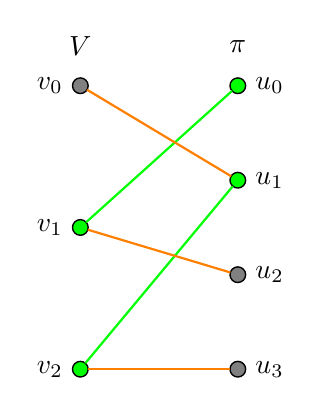
\begin{tikzpicture}
          \node at (0,1.5){$V$};
          \node at (2,1.5){$\pi$};
          \GraphInit[vstyle=Classic];
          \SetVertexNormal[MinSize=1pt,FillColor=black]
          
          \SetVertexNormal[MinSize=1pt,FillColor=orange]
          
          \SetVertexNormal[MinSize=1pt,FillColor=blue]
          
          \SetVertexNormal[MinSize=1pt,FillColor=green]
          \Vertex[Math,x=0,y=-0.8,Lpos=180]{v_1};
          \Vertex[Math,x=0,y=-2.6,Lpos=180]{v_2};
          \Vertex[Math,x=2,y=1]{u_0};
          \Vertex[Math,x=2,y=-0.2]{u_1};
          
          \SetVertexNormal[MinSize=1pt,FillColor=gray]
          \Vertex[Math,x=0,y=1,Lpos=180]{v_0};
          \Vertex[Math,x=2,y=-1.4]{u_2};
          \Vertex[Math,x=2,y=-2.6]{u_3};
          
          % matching edges
          \tikzset{EdgeStyle/.append style = {green}};
          \Edge(v_1)(u_0);
          \Edge(v_2)(u_1);
          
          % discarded eges
          \tikzset{EdgeStyle/.append style = {orange}};
          \Edge(v_0)(u_1);
          \Edge(v_1)(u_2);
          \Edge(v_2)(u_3);
        \end{tikzpicture}}
    \end{column}
  \end{columns}
  \onslide<3->
  \begin{block}{Competitive ratio for OBM}
    \only<-3>{\[
      \min_G \min_\pi \frac{\card{\mathcal{A}(G,\pi)}}{\card{M}}
    \]}
    \only<4->{\[
      \min_G \min_\pi \frac{\mathbb{E}\big[\card{\mathcal{A}(G,\pi)}\big]}{\card{M}}
    \]}
    where $M$ is a maximum cardinality matching in $G$.
  \end{block}
  \note{
    \begin{itemize}
      \item as seen before: Hopcroft-Karp for max-card matching
      \item deterministic \textrightarrow{} competitive ratio of $\frac{1}{2}$
      \item add randomiztion \textrightarrow{} consider expected size
    \end{itemize}
  }
\end{frame}

\begin{frame}
  \frametitle{RANKING}
  \onslide<+->
  \begin{itemize}
    \item simple randomized algorithm due to Karp, Vazirani, and Vazirani~\cite{karp1990}
  \end{itemize}
  \onslide<+->
  \begin{columns}
    \begin{column}{.3\textwidth}
      \only<-2>{
        \adjustbox{scale=0.8}{
          \begin{tikzpicture}
            \node at (0,0.5){$V$};
            \node at (2,0.5){$\pi$};
            \GraphInit[vstyle=Classic];
               
            \SetVertexNormal[MinSize=1pt,FillColor=black]
            \Vertex[Math,Lpos=180,x=0,y=0]{v_0};
            \Vertex[Math,Lpos=180,x=0,y=-1.2]{v_1};
            \Vertex[Math,Lpos=180,x=0,y=-2.4]{v_2};
            \Vertex[Math,Lpos=180,x=0,y=-3.6]{v_3};
          \end{tikzpicture}
        }
      }%
      \only<3>{
        \adjustbox{scale=0.8}{
          \begin{tikzpicture}
            \node at (0,0.5){\phantom{$V$}};
            \node at (0,0.5){$\sigma$};
            \node at (2,0.5){$\pi$};
            \GraphInit[vstyle=Classic];
               
            \SetVertexNormal[MinSize=1pt,FillColor=black]
            \Vertex[Math,Lpos=180,x=0,y=0]{v_2};
            \Vertex[Math,Lpos=180,x=0,y=-1.2]{v_3};
            \Vertex[Math,Lpos=180,x=0,y=-2.4]{v_1};
            \Vertex[Math,Lpos=180,x=0,y=-3.6]{v_0};
          \end{tikzpicture}
         }
      }%
      \only<4>{
        \adjustbox{scale=0.8}{
          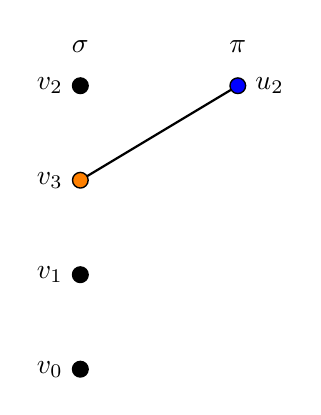
\begin{tikzpicture}
            \node at (0,0.5){\phantom{$V$}};
            \node at (0,0.5){$\sigma$};
            \node at (2,0.5){$\pi$};
            \GraphInit[vstyle=Classic];
               
            \SetVertexNormal[MinSize=1pt,FillColor=black]
            \Vertex[Math,Lpos=180,x=0,y=0]{v_2};
            \Vertex[Math,Lpos=180,x=0,y=-2.4]{v_1};
            \Vertex[Math,Lpos=180,x=0,y=-3.6]{v_0};
            
            \SetVertexNormal[MinSize=1pt,FillColor=blue]
            \Vertex[Math,x=2,y=0]{u_2};
            
            \SetVertexNormal[MinSize=1pt,FillColor=orange]
            \Vertex[Math,Lpos=180,x=0,y=-1.2]{v_3};
            
            \Edge(u_2)(v_3);
          \end{tikzpicture}
        }
      }%
      \only<5>{
        \adjustbox{scale=0.8}{
          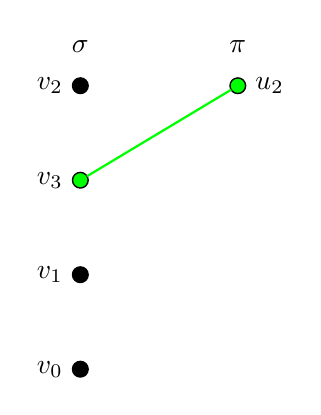
\begin{tikzpicture}
            \node at (0,0.5){\phantom{$V$}};
            \node at (0,0.5){$\sigma$};
            \node at (2,0.5){$\pi$};
            \GraphInit[vstyle=Classic];
               
            \SetVertexNormal[MinSize=1pt,FillColor=black]
            \Vertex[Math,Lpos=180,x=0,y=0]{v_2};
            \Vertex[Math,Lpos=180,x=0,y=-2.4]{v_1};
            \Vertex[Math,Lpos=180,x=0,y=-3.6]{v_0};
            
            \SetVertexNormal[MinSize=1pt,FillColor=blue]
            
            \SetVertexNormal[MinSize=1pt,FillColor=orange]
            
            \SetVertexNormal[MinSize=1pt,FillColor=green]
            \Vertex[Math,x=2,y=0]{u_2};            
            \Vertex[Math,Lpos=180,x=0,y=-1.2]{v_3};
            
            \tikzset{EdgeStyle/.append style={green}};
            \Edge(u_2)(v_3);
          \end{tikzpicture}
        }
      }%
      \only<6>{
        \adjustbox{scale=0.8}{
          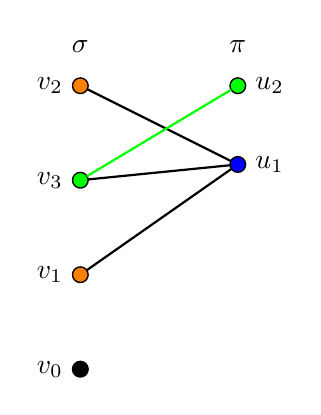
\begin{tikzpicture}
            \node at (0,0.5){\phantom{$V$}};
            \node at (0,0.5){$\sigma$};
            \node at (2,0.5){$\pi$};
            \GraphInit[vstyle=Classic];
               
            \SetVertexNormal[MinSize=1pt,FillColor=black]
            \Vertex[Math,Lpos=180,x=0,y=-3.6]{v_0};
            
            \SetVertexNormal[MinSize=1pt,FillColor=blue]
            \Vertex[Math,x=2,y=-1]{u_1};
            
            \SetVertexNormal[MinSize=1pt,FillColor=orange]
            \Vertex[Math,Lpos=180,x=0,y=0]{v_2};
            \Vertex[Math,Lpos=180,x=0,y=-2.4]{v_1};
            
            \SetVertexNormal[MinSize=1pt,FillColor=green]
            \Vertex[Math,x=2,y=0]{u_2};            
            \Vertex[Math,Lpos=180,x=0,y=-1.2]{v_3};
            
            \Edge(u_1)(v_2);
            \Edge(u_1)(v_3);
            \Edge(u_1)(v_1);
            
            \tikzset{EdgeStyle/.append style={green}};
            \Edge(u_2)(v_3);
          \end{tikzpicture}
        }
      }%
      \only<7>{
        \adjustbox{scale=0.8}{
          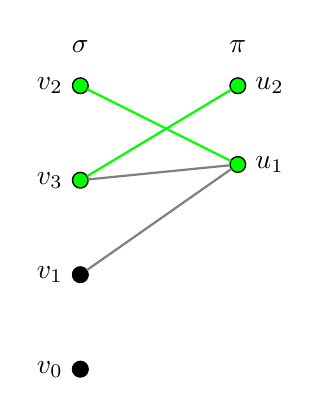
\begin{tikzpicture}
            \node at (0,0.5){\phantom{$V$}};
            \node at (0,0.5){$\sigma$};
            \node at (2,0.5){$\pi$};
            \GraphInit[vstyle=Classic];
               
            \SetVertexNormal[MinSize=1pt,FillColor=black]
            \Vertex[Math,Lpos=180,x=0,y=-2.4]{v_1};
            \Vertex[Math,Lpos=180,x=0,y=-3.6]{v_0};
            
            \SetVertexNormal[MinSize=1pt,FillColor=blue]
                        
            \SetVertexNormal[MinSize=1pt,FillColor=orange]
            
            \SetVertexNormal[MinSize=1pt,FillColor=green]
            \Vertex[Math,x=2,y=0]{u_2};            
            \Vertex[Math,Lpos=180,x=0,y=-1.2]{v_3};
            \Vertex[Math,x=2,y=-1]{u_1};
            \Vertex[Math,Lpos=180,x=0,y=0]{v_2};
                        
            \tikzset{EdgeStyle/.append style={green}};
            \Edge(u_2)(v_3);
            \Edge(u_1)(v_2);
            
            \tikzset{EdgeStyle/.append style={gray}};
            \Edge(u_1)(v_3);
            \Edge(u_1)(v_1);
          \end{tikzpicture}
        }
      }%
      \only<8>{
        \adjustbox{scale=0.8}{
          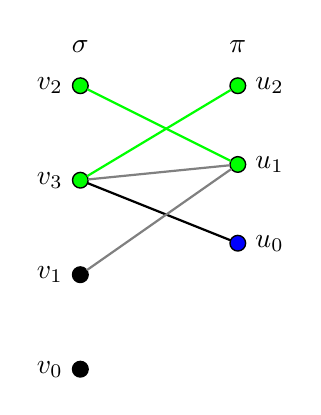
\begin{tikzpicture}
            \node at (0,0.5){\phantom{$V$}};
            \node at (0,0.5){$\sigma$};
            \node at (2,0.5){$\pi$};
            \GraphInit[vstyle=Classic];
               
            \SetVertexNormal[MinSize=1pt,FillColor=black]
            \Vertex[Math,Lpos=180,x=0,y=-2.4]{v_1};
            \Vertex[Math,Lpos=180,x=0,y=-3.6]{v_0};
            
            \SetVertexNormal[MinSize=1pt,FillColor=blue]
            \Vertex[Math,x=2,y=-2]{u_0};
            
            \SetVertexNormal[MinSize=1pt,FillColor=orange]
            
            \SetVertexNormal[MinSize=1pt,FillColor=green]
            \Vertex[Math,x=2,y=0]{u_2};            
            \Vertex[Math,Lpos=180,x=0,y=-1.2]{v_3};
            \Vertex[Math,x=2,y=-1]{u_1};
            \Vertex[Math,Lpos=180,x=0,y=0]{v_2};
            
            \Edge(u_0)(v_3);
                        
            \tikzset{EdgeStyle/.append style={green}};
            \Edge(u_2)(v_3);
            \Edge(u_1)(v_2);
            
            \tikzset{EdgeStyle/.append style={gray}};
            \Edge(u_1)(v_3);
            \Edge(u_1)(v_1);
          \end{tikzpicture}
        }
      }%
      \only<9>{
        \adjustbox{scale=0.8}{
          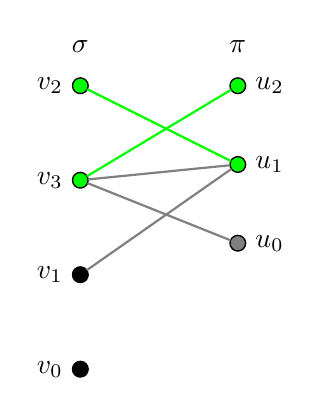
\begin{tikzpicture}
            \node at (0,0.5){\phantom{$V$}};
            \node at (0,0.5){$\sigma$};
            \node at (2,0.5){$\pi$};
            \GraphInit[vstyle=Classic];
               
            \SetVertexNormal[MinSize=1pt,FillColor=black]
            \Vertex[Math,Lpos=180,x=0,y=-2.4]{v_1};
            \Vertex[Math,Lpos=180,x=0,y=-3.6]{v_0};
            
            \SetVertexNormal[MinSize=1pt,FillColor=blue]
            
            \SetVertexNormal[MinSize=1pt,FillColor=orange]
            
            \SetVertexNormal[MinSize=1pt,FillColor=green]
            \Vertex[Math,x=2,y=0]{u_2};            
            \Vertex[Math,Lpos=180,x=0,y=-1.2]{v_3};
            \Vertex[Math,x=2,y=-1]{u_1};
            \Vertex[Math,Lpos=180,x=0,y=0]{v_2};
            
            \SetVertexNormal[MinSize=1pt,FillColor=gray]
            \Vertex[Math,x=2,y=-2]{u_0};
                        
            \tikzset{EdgeStyle/.append style={green}};
            \Edge(u_2)(v_3);
            \Edge(u_1)(v_2);
            
            \tikzset{EdgeStyle/.append style={gray}};
            \Edge(u_1)(v_3);
            \Edge(u_1)(v_1);
            \Edge(u_0)(v_3);
          \end{tikzpicture}
        }
      }%
      \only<10>{
        \adjustbox{scale=0.8}{
          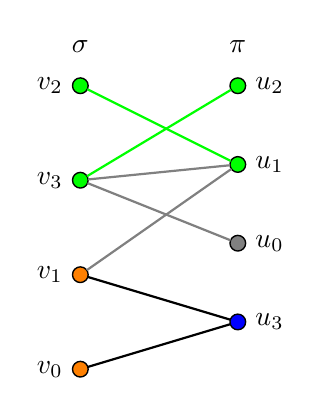
\begin{tikzpicture}
            \node at (0,0.5){\phantom{$V$}};
            \node at (0,0.5){$\sigma$};
            \node at (2,0.5){$\pi$};
            \GraphInit[vstyle=Classic];
               
            \SetVertexNormal[MinSize=1pt,FillColor=black]
            
            \SetVertexNormal[MinSize=1pt,FillColor=blue]
            \Vertex[Math,x=2,y=-3]{u_3};
            
            \SetVertexNormal[MinSize=1pt,FillColor=orange]
            \Vertex[Math,Lpos=180,x=0,y=-2.4]{v_1};
            \Vertex[Math,Lpos=180,x=0,y=-3.6]{v_0};
            
            \SetVertexNormal[MinSize=1pt,FillColor=green]
            \Vertex[Math,x=2,y=0]{u_2};            
            \Vertex[Math,Lpos=180,x=0,y=-1.2]{v_3};
            \Vertex[Math,x=2,y=-1]{u_1};
            \Vertex[Math,Lpos=180,x=0,y=0]{v_2};
            
            \SetVertexNormal[MinSize=1pt,FillColor=gray]
            \Vertex[Math,x=2,y=-2]{u_0};
            
            \Edge(u_3)(v_1);
            \Edge(u_3)(v_0);
                        
            \tikzset{EdgeStyle/.append style={green}};
            \Edge(u_2)(v_3);
            \Edge(u_1)(v_2);
            
            \tikzset{EdgeStyle/.append style={gray}};
            \Edge(u_1)(v_3);
            \Edge(u_1)(v_1);
            \Edge(u_0)(v_3);
          \end{tikzpicture}
        }
      }%
      \only<11->{
        \adjustbox{scale=0.8}{
          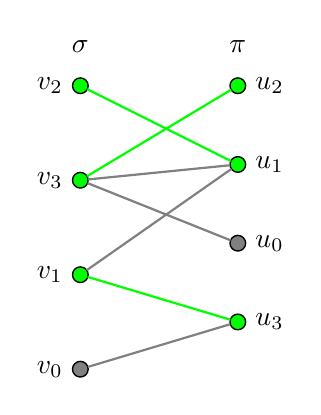
\begin{tikzpicture}
            \node at (0,0.5){\phantom{$V$}};
            \node at (0,0.5){$\sigma$};
            \node at (2,0.5){$\pi$};
            \GraphInit[vstyle=Classic];
               
            \SetVertexNormal[MinSize=1pt,FillColor=black]
            
            \SetVertexNormal[MinSize=1pt,FillColor=blue]
            
            \SetVertexNormal[MinSize=1pt,FillColor=orange]
            
            \SetVertexNormal[MinSize=1pt,FillColor=green]
            \Vertex[Math,x=2,y=0]{u_2};            
            \Vertex[Math,Lpos=180,x=0,y=-1.2]{v_3};
            \Vertex[Math,x=2,y=-1]{u_1};
            \Vertex[Math,Lpos=180,x=0,y=0]{v_2};
            \Vertex[Math,x=2,y=-3]{u_3};
            \Vertex[Math,Lpos=180,x=0,y=-2.4]{v_1};
            
            \SetVertexNormal[MinSize=1pt,FillColor=gray]
            \Vertex[Math,x=2,y=-2]{u_0};
            \Vertex[Math,Lpos=180,x=0,y=-3.6]{v_0};
                                    
            \tikzset{EdgeStyle/.append style={green}};
            \Edge(u_2)(v_3);
            \Edge(u_1)(v_2);
            \Edge(u_3)(v_1);
            
            \tikzset{EdgeStyle/.append style={gray}};
            \Edge(u_1)(v_3);
            \Edge(u_1)(v_1);
            \Edge(u_0)(v_3);
            \Edge(u_3)(v_0);
          \end{tikzpicture}
        }
      }%
    \end{column}
    \begin{column}{.65\textwidth}
      \begin{algorithm}[H]
        \footnotesize
        \DontPrintSemicolon
        \Init{Choose a random permutation (ranking) $\sigma$ of $V$}
        \Online{}
        \Arrival{$u \in U$}{
          $N(u) \gets \text{set of unmatched neighbors of }u$\\
          \If{$N(u) \neq \emptyset$}{
            match $u$ to the vertex $v \in N(u)$ that minimizes $\sigma(v)$
          }
        }
      \end{algorithm}
    \end{column}
  \end{columns}
  \onslide<12->
  \begin{itemize}
    \item competitive ratio of $1 - \frac{1}{e}$ (best possible)
  \end{itemize}
\end{frame}

\begin{frame}
  \frametitle{Formalization Outline}
  \note{
    \begin{itemize}
      \item follow simplified proof
      \item prove competitive ratio $1-\frac{1}{e}$, not that it's best possible
      \item Combinatorics: fix graph, arrival and ranking
      \item Prob: use material from comb in randomized setting
      \item lower bound competitive ratio depending on $\card{M}$
      \item when $\card{M} \to \infty$, bound goes to $1-\frac{1}{e}$
      \item focus on combinatorics, a bit on probabilities, skip limit
    \end{itemize}
  }
  \begin{itemize}[<+->]
    \item formalization follows proof due to Birnbaum \& Mathieu~\cite{birnbaum2008}
    \item three parts
    \begin{enumerate}
      \item \only<3-5>{Combinatorics} \only<6->{\textbf{Combinatorics}}
      \item Probability theory
      \item Competitive ratio in the limit
    \end{enumerate}
  \end{itemize}
\end{frame}

\section{Combinatorics}

\begin{frame}
  \frametitle{Reducing Analysis to Graphs with Perfect Matching}
  \note{
    \begin{itemize}
      \item perfect matching gives additional structure we can exploit in randomized analysis
      \item consider what happens when removing a single vertex (how do the matchings differ
        when keeping the same arrival order and ranking)
      \item cascading \textrightarrow{} $u_3$ is in same situation as $u_1$
      \item not necessarily always two edges in symm.\ diff
      \item consequence: matchings can only shrink towards "perfect matching graph"
    \end{itemize}
  }
  \begin{itemize}[<+->]
    \item original paper (and earlier simplifications) assume $G$ has a perfect matching
    \item Birnbaum \& Mathieu state a lemma which allows to
      generalize to arbitrary graphs:
  \end{itemize}
  \begin{columns}
    \begin{column}{.3\textwidth}
      \onslide<3->{
        \adjustbox{scale=0.8}{
          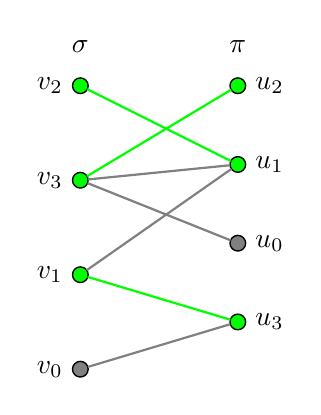
\begin{tikzpicture}
            \node at (0,0.5){\phantom{$V$}};
            \node at (0,0.5){$\sigma$};
            \node at (2,0.5){$\pi$};
            \GraphInit[vstyle=Classic];
               
            \SetVertexNormal[MinSize=1pt,FillColor=black]
            
            \SetVertexNormal[MinSize=1pt,FillColor=blue]
            
            \SetVertexNormal[MinSize=1pt,FillColor=orange]
            
            \SetVertexNormal[MinSize=1pt,FillColor=green]
            \Vertex[Math,x=2,y=0]{u_2};            
            \Vertex[Math,Lpos=180,x=0,y=-1.2]{v_3};
            \Vertex[Math,x=2,y=-1]{u_1};
            \Vertex[Math,Lpos=180,x=0,y=0]{v_2};
            \Vertex[Math,x=2,y=-3]{u_3};
            \Vertex[Math,Lpos=180,x=0,y=-2.4]{v_1};
            
            \SetVertexNormal[MinSize=1pt,FillColor=gray]
            \Vertex[Math,x=2,y=-2]{u_0};
            \Vertex[Math,Lpos=180,x=0,y=-3.6]{v_0};
                                    
            \tikzset{EdgeStyle/.append style={green}};
            \Edge(u_2)(v_3);
            \Edge(u_1)(v_2);
            \Edge(u_3)(v_1);
            
            \tikzset{EdgeStyle/.append style={gray}};
            \Edge(u_1)(v_3);
            \Edge(u_1)(v_1);
            \Edge(u_0)(v_3);
            \Edge(u_3)(v_0);
          \end{tikzpicture}
        }
      }%
    \end{column}
    \begin{column}{.3\textwidth}
      \only<3-4>{
        \adjustbox{scale=0.8}{
          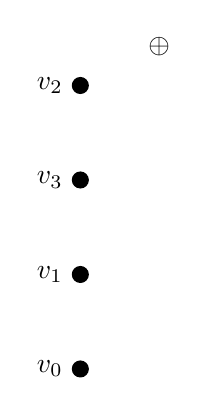
\begin{tikzpicture}
            \node at (1,0.5){$\oplus$};
            \GraphInit[vstyle=Classic];
               
            \SetVertexNormal[MinSize=1pt,FillColor=black]
            \Vertex[Math,Lpos=180,x=0,y=0]{v_2};
            \Vertex[Math,Lpos=180,x=0,y=-1.2]{v_3};
            \Vertex[Math,Lpos=180,x=0,y=-2.4]{v_1};
            \Vertex[Math,Lpos=180,x=0,y=-3.6]{v_0};
          \end{tikzpicture}
        }
      }%
      \only<5-6>{
        \adjustbox{scale=0.8}{
          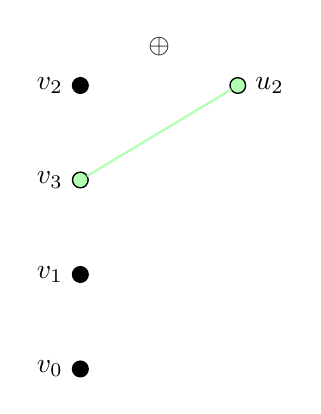
\begin{tikzpicture}
            \node at (1,0.5){$\oplus$};
            \GraphInit[vstyle=Classic];
               
            \SetVertexNormal[MinSize=1pt,FillColor=black]
            \Vertex[Math,Lpos=180,x=0,y=0]{v_2};
            \Vertex[Math,Lpos=180,x=0,y=-2.4]{v_1};
            \Vertex[Math,Lpos=180,x=0,y=-3.6]{v_0};
            
            \SetVertexNormal[MinSize=1pt,FillColor=green!30]
            \Vertex[Math,Lpos=180,x=0,y=-1.2]{v_3};
            \Vertex[Math,x=2,y=0]{u_2};
            
            \tikzset{EdgeStyle/.append style={green!30}};
            \Edge(v_3)(u_2);
          
          \end{tikzpicture}
        }
      }%
      \only<7-8>{
        \adjustbox{scale=0.8}{
          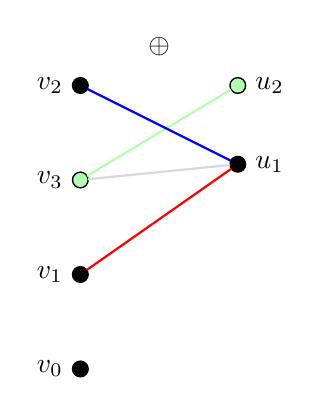
\begin{tikzpicture}
            \node at (1,0.5){$\oplus$};
            \GraphInit[vstyle=Classic];
               
            \SetVertexNormal[MinSize=1pt,FillColor=black]
            \Vertex[Math,Lpos=180,x=0,y=0]{v_2};
            \Vertex[Math,Lpos=180,x=0,y=-2.4]{v_1};
            \Vertex[Math,Lpos=180,x=0,y=-3.6]{v_0};
            \Vertex[Math,x=2,y=-1]{u_1};
            
            \SetVertexNormal[MinSize=1pt,FillColor=green!30]
            \Vertex[Math,Lpos=180,x=0,y=-1.2]{v_3};
            \Vertex[Math,x=2,y=0]{u_2};
            
            \tikzset{EdgeStyle/.append style={green!30}};
            \Edge(v_3)(u_2);
            
            \tikzset{EdgeStyle/.append style={gray!30}};
            \Edge(v_3)(u_1);
            
            \tikzset{EdgeStyle/.append style={blue}};
            \Edge(v_2)(u_1);
            
            \tikzset{EdgeStyle/.append style={red}};
            \Edge(v_1)(u_1);            
          \end{tikzpicture}
        }
      }%
      \only<9-10>{
        \adjustbox{scale=0.8}{
          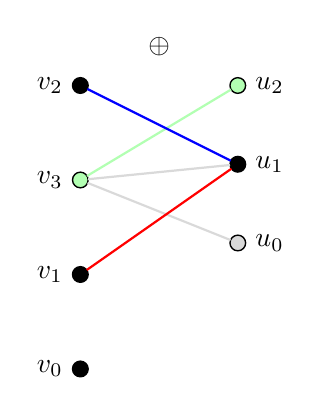
\begin{tikzpicture}
            \node at (1,0.5){$\oplus$};
            \GraphInit[vstyle=Classic];
               
            \SetVertexNormal[MinSize=1pt,FillColor=black]
            \Vertex[Math,Lpos=180,x=0,y=0]{v_2};
            \Vertex[Math,Lpos=180,x=0,y=-2.4]{v_1};
            \Vertex[Math,Lpos=180,x=0,y=-3.6]{v_0};
            \Vertex[Math,x=2,y=-1]{u_1};
            
            \SetVertexNormal[MinSize=1pt,FillColor=green!30]
            \Vertex[Math,Lpos=180,x=0,y=-1.2]{v_3};
            \Vertex[Math,x=2,y=0]{u_2};
            
            \SetVertexNormal[MinSize=1pt,FillColor=gray!30]
            \Vertex[Math,x=2,y=-2]{u_0}
            
            \tikzset{EdgeStyle/.append style={green!30}};
            \Edge(v_3)(u_2);
            
            \tikzset{EdgeStyle/.append style={gray!30}};
            \Edge(v_3)(u_1);
            \Edge(v_3)(u_0);
            
            \tikzset{EdgeStyle/.append style={blue}};
            \Edge(v_2)(u_1);
            
            \tikzset{EdgeStyle/.append style={red}};
            \Edge(v_1)(u_1);            
          \end{tikzpicture}
        }
      }%
      \only<11>{
        \adjustbox{scale=0.8}{
          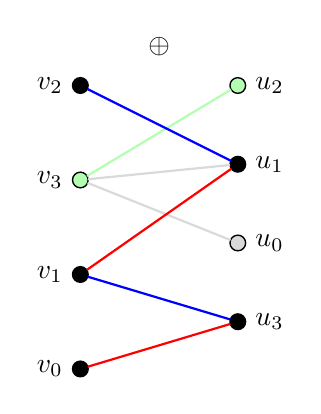
\begin{tikzpicture}
            \node at (1,0.5){$\oplus$};
            \GraphInit[vstyle=Classic];
               
            \SetVertexNormal[MinSize=1pt,FillColor=black]
            \Vertex[Math,Lpos=180,x=0,y=0]{v_2};
            \Vertex[Math,Lpos=180,x=0,y=-2.4]{v_1};
            \Vertex[Math,Lpos=180,x=0,y=-3.6]{v_0};
            \Vertex[Math,x=2,y=-1]{u_1};
            \Vertex[Math,x=2,y=-3]{u_3};
            
            \SetVertexNormal[MinSize=1pt,FillColor=green!30]
            \Vertex[Math,Lpos=180,x=0,y=-1.2]{v_3};
            \Vertex[Math,x=2,y=0]{u_2};
            
            \SetVertexNormal[MinSize=1pt,FillColor=gray!30]
            \Vertex[Math,x=2,y=-2]{u_0}
            
            \tikzset{EdgeStyle/.append style={green!30}};
            \Edge(v_3)(u_2);
            
            \tikzset{EdgeStyle/.append style={gray!30}};
            \Edge(v_3)(u_1);
            \Edge(v_3)(u_0);
            
            \tikzset{EdgeStyle/.append style={blue}};
            \Edge(v_2)(u_1);
            \Edge(v_1)(u_3);
            
            \tikzset{EdgeStyle/.append style={red}};
            \Edge(v_1)(u_1);
            \Edge(v_0)(u_3);            
          \end{tikzpicture}
        }
      }%
      \only<12->{
        \adjustbox{scale=0.8}{
          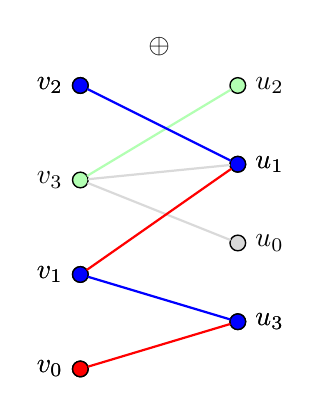
\begin{tikzpicture}
            \node at (1,0.5){$\oplus$};
            \GraphInit[vstyle=Classic];
               
            \SetVertexNormal[MinSize=1pt,FillColor=black]
            \Vertex[Math,Lpos=180,x=0,y=0]{v_2};
            \Vertex[Math,Lpos=180,x=0,y=-2.4]{v_1};
            \Vertex[Math,Lpos=180,x=0,y=-3.6]{v_0};
            \Vertex[Math,x=2,y=-1]{u_1};
            \Vertex[Math,x=2,y=-3]{u_3};
            
            \SetVertexNormal[MinSize=1pt,FillColor=blue]
            \Vertex[Math,Lpos=180,x=0,y=0]{v_2};
            \Vertex[Math,Lpos=180,x=0,y=-2.4]{v_1};
            \Vertex[Math,x=2,y=-1]{u_1};
            \Vertex[Math,x=2,y=-3]{u_3};
            
            \SetVertexNormal[MinSize=1pt,FillColor=red]
            \Vertex[Math,Lpos=180,x=0,y=-3.6]{v_0};
            
            \SetVertexNormal[MinSize=1pt,FillColor=green!30]
            \Vertex[Math,Lpos=180,x=0,y=-1.2]{v_3};
            \Vertex[Math,x=2,y=0]{u_2};
            
            \SetVertexNormal[MinSize=1pt,FillColor=gray!30]
            \Vertex[Math,x=2,y=-2]{u_0}
            
            \tikzset{EdgeStyle/.append style={green!30}};
            \Edge(v_3)(u_2);
            
            \tikzset{EdgeStyle/.append style={gray!30}};
            \Edge(v_3)(u_1);
            \Edge(v_3)(u_0);
            
            \tikzset{EdgeStyle/.append style={blue}};
            \Edge(v_2)(u_1);
            \Edge(v_1)(u_3);
            
            \tikzset{EdgeStyle/.append style={red}};
            \Edge(v_1)(u_1);
            \Edge(v_0)(u_3);            
          \end{tikzpicture}
        }
      }%
    \end{column}
    \begin{column}{.3\textwidth}
      \only<3>{
        \adjustbox{scale=0.8}{
          \begin{tikzpicture}
            \node at (0,0.5){\phantom{$V$}};
            \node at (0,0.5){$\sigma'$};
            \node at (2,0.5){$\pi$};
            \GraphInit[vstyle=Classic];
               
            \SetVertexNormal[MinSize=1pt,FillColor=black]
            \Vertex[Math,Lpos=180,x=0,y=-1.2]{v_3};
            \Vertex[Math,Lpos=180,x=0,y=-2.4]{v_1};
            \Vertex[Math,Lpos=180,x=0,y=-3.6]{v_0};
          \end{tikzpicture}
        }
      }%
      \only<4>{
        \adjustbox{scale=0.8}{
          \begin{tikzpicture}
            \node at (0,0.5){\phantom{$V$}};
            \node at (0,0.5){$\sigma'$};
            \node at (2,0.5){$\pi$};
            \GraphInit[vstyle=Classic];
               
            \SetVertexNormal[MinSize=1pt,FillColor=black]
            \Vertex[Math,Lpos=180,x=0,y=-2.4]{v_1};
            \Vertex[Math,Lpos=180,x=0,y=-3.6]{v_0};
            
            \SetVertexNormal[MinSize=1pt,FillColor=blue]
            \Vertex[Math,x=2,y=0]{u_2};
            
            \SetVertexNormal[MinSize=1pt,FillColor=orange]
            \Vertex[Math,Lpos=180,x=0,y=-1.2]{v_3};
            
            \Edge(u_2)(v_3);
          \end{tikzpicture}
        }
      }%
      \only<5>{
        \adjustbox{scale=0.8}{
          \begin{tikzpicture}
            \node at (0,0.5){\phantom{$V$}};
            \node at (0,0.5){$\sigma'$};
            \node at (2,0.5){$\pi$};
            \GraphInit[vstyle=Classic];
               
            \SetVertexNormal[MinSize=1pt,FillColor=black]
            \Vertex[Math,Lpos=180,x=0,y=-2.4]{v_1};
            \Vertex[Math,Lpos=180,x=0,y=-3.6]{v_0};
            
            \SetVertexNormal[MinSize=1pt,FillColor=blue]
            
            \SetVertexNormal[MinSize=1pt,FillColor=orange]
            
            \SetVertexNormal[MinSize=1pt,FillColor=green]
            \Vertex[Math,x=2,y=0]{u_2};            
            \Vertex[Math,Lpos=180,x=0,y=-1.2]{v_3};
            
            \tikzset{EdgeStyle/.append style={green}};
            \Edge(u_2)(v_3);
          \end{tikzpicture}
        }
      }%
      \only<6>{
        \adjustbox{scale=0.8}{
          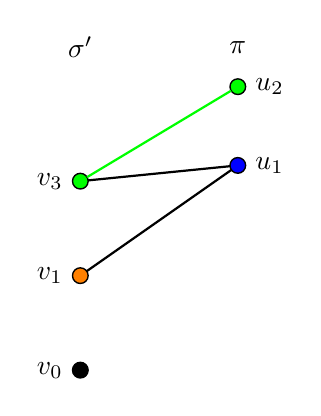
\begin{tikzpicture}
            \node at (0,0.5){\phantom{$V$}};
            \node at (0,0.5){$\sigma'$};
            \node at (2,0.5){$\pi$};
            \GraphInit[vstyle=Classic];
               
            \SetVertexNormal[MinSize=1pt,FillColor=black]
            \Vertex[Math,Lpos=180,x=0,y=-3.6]{v_0};
            
            \SetVertexNormal[MinSize=1pt,FillColor=blue]
            \Vertex[Math,x=2,y=-1]{u_1};
            
            \SetVertexNormal[MinSize=1pt,FillColor=orange]
            \Vertex[Math,Lpos=180,x=0,y=-2.4]{v_1};
            
            \SetVertexNormal[MinSize=1pt,FillColor=green]
            \Vertex[Math,x=2,y=0]{u_2};            
            \Vertex[Math,Lpos=180,x=0,y=-1.2]{v_3};
            
            \Edge(u_1)(v_3);
            \Edge(u_1)(v_1);
            
            \tikzset{EdgeStyle/.append style={green}};
            \Edge(u_2)(v_3);
          \end{tikzpicture}
        }
      }%
      \only<7>{
        \adjustbox{scale=0.8}{
          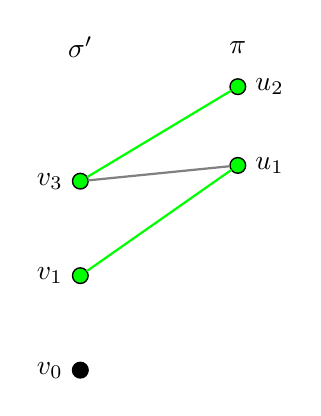
\begin{tikzpicture}
            \node at (0,0.5){\phantom{$V$}};
            \node at (0,0.5){$\sigma'$};
            \node at (2,0.5){$\pi$};
            \GraphInit[vstyle=Classic];
               
            \SetVertexNormal[MinSize=1pt,FillColor=black]
            \Vertex[Math,Lpos=180,x=0,y=-3.6]{v_0};
            
            \SetVertexNormal[MinSize=1pt,FillColor=blue]
            
            \SetVertexNormal[MinSize=1pt,FillColor=orange]
            
            \SetVertexNormal[MinSize=1pt,FillColor=green]
            \Vertex[Math,x=2,y=0]{u_2};            
            \Vertex[Math,Lpos=180,x=0,y=-1.2]{v_3};
            \Vertex[Math,x=2,y=-1]{u_1};
            \Vertex[Math,Lpos=180,x=0,y=-2.4]{v_1};
                        
            \tikzset{EdgeStyle/.append style={green}};
            \Edge(u_2)(v_3);
            \Edge(u_1)(v_1);
            
            \tikzset{EdgeStyle/.append style={gray}};
            \Edge(u_1)(v_3);
          \end{tikzpicture}
        }
      }%
      \only<8>{
        \adjustbox{scale=0.8}{
          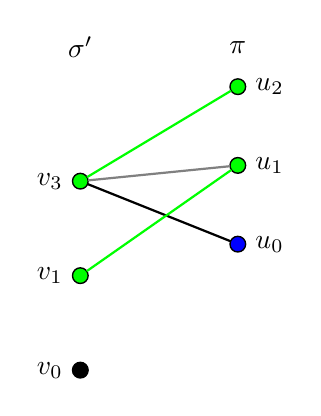
\begin{tikzpicture}
            \node at (0,0.5){\phantom{$V$}};
            \node at (0,0.5){$\sigma'$};
            \node at (2,0.5){$\pi$};
            \GraphInit[vstyle=Classic];
               
            \SetVertexNormal[MinSize=1pt,FillColor=black]
            \Vertex[Math,Lpos=180,x=0,y=-3.6]{v_0};
            
            \SetVertexNormal[MinSize=1pt,FillColor=blue]
            \Vertex[Math,x=2,y=-2]{u_0};
            
            \SetVertexNormal[MinSize=1pt,FillColor=orange]
            
            \SetVertexNormal[MinSize=1pt,FillColor=green]
            \Vertex[Math,x=2,y=0]{u_2};            
            \Vertex[Math,Lpos=180,x=0,y=-1.2]{v_3};
            \Vertex[Math,x=2,y=-1]{u_1};
            \Vertex[Math,Lpos=180,x=0,y=-2.4]{v_1};
            
            \Edge(v_3)(u_0);
                        
            \tikzset{EdgeStyle/.append style={green}};
            \Edge(u_2)(v_3);
            \Edge(u_1)(v_1);
            
            \tikzset{EdgeStyle/.append style={gray}};
            \Edge(u_1)(v_3);
          \end{tikzpicture}
        }
      }%
      \only<9>{
        \adjustbox{scale=0.8}{
          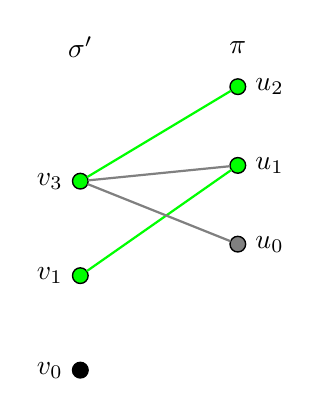
\begin{tikzpicture}
            \node at (0,0.5){\phantom{$V$}};
            \node at (0,0.5){$\sigma'$};
            \node at (2,0.5){$\pi$};
            \GraphInit[vstyle=Classic];
               
            \SetVertexNormal[MinSize=1pt,FillColor=black]
            \Vertex[Math,Lpos=180,x=0,y=-3.6]{v_0};
            
            \SetVertexNormal[MinSize=1pt,FillColor=blue]
            
            \SetVertexNormal[MinSize=1pt,FillColor=orange]
            
            \SetVertexNormal[MinSize=1pt,FillColor=green]
            \Vertex[Math,x=2,y=0]{u_2};            
            \Vertex[Math,Lpos=180,x=0,y=-1.2]{v_3};
            \Vertex[Math,x=2,y=-1]{u_1};
            \Vertex[Math,Lpos=180,x=0,y=-2.4]{v_1};
            
            \SetVertexNormal[MinSize=1pt,FillColor=gray]
            \Vertex[Math,x=2,y=-2]{u_0};
            
                        
            \tikzset{EdgeStyle/.append style={green}};
            \Edge(u_2)(v_3);
            \Edge(u_1)(v_1);
            
            \tikzset{EdgeStyle/.append style={gray}};
            \Edge(u_1)(v_3);
            \Edge(v_3)(u_0);
          \end{tikzpicture}
        }
      }%
      \only<10>{
        \adjustbox{scale=0.8}{
          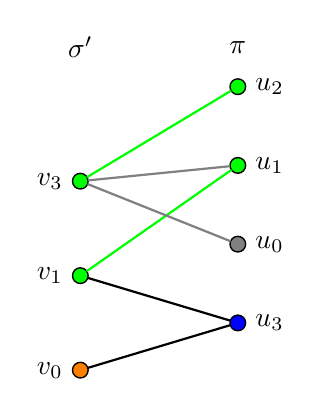
\begin{tikzpicture}
            \node at (0,0.5){\phantom{$V$}};
            \node at (0,0.5){$\sigma'$};
            \node at (2,0.5){$\pi$};
            \GraphInit[vstyle=Classic];
               
            \SetVertexNormal[MinSize=1pt,FillColor=black]
            
            \SetVertexNormal[MinSize=1pt,FillColor=blue]
            \Vertex[Math,x=2,y=-3]{u_3};
            
            \SetVertexNormal[MinSize=1pt,FillColor=orange]
            \Vertex[Math,Lpos=180,x=0,y=-3.6]{v_0};
            
            \SetVertexNormal[MinSize=1pt,FillColor=green]
            \Vertex[Math,x=2,y=0]{u_2};            
            \Vertex[Math,Lpos=180,x=0,y=-1.2]{v_3};
            \Vertex[Math,x=2,y=-1]{u_1};
            \Vertex[Math,Lpos=180,x=0,y=-2.4]{v_1};
            
            \SetVertexNormal[MinSize=1pt,FillColor=gray]
            \Vertex[Math,x=2,y=-2]{u_0};
            
            \Edge(v_0)(u_3);
            \Edge(v_1)(u_3);
            
            \tikzset{EdgeStyle/.append style={green}};
            \Edge(u_2)(v_3);
            \Edge(u_1)(v_1);
            
            \tikzset{EdgeStyle/.append style={gray}};
            \Edge(u_1)(v_3);
            \Edge(v_3)(u_0);
          \end{tikzpicture}
        }
      }%
      \only<11->{
        \adjustbox{scale=0.8}{
          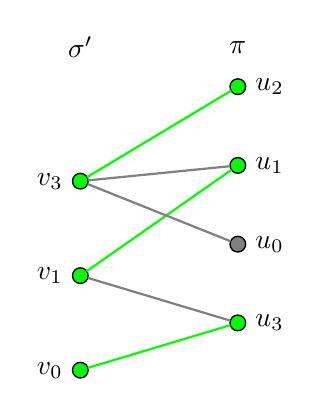
\begin{tikzpicture}
            \node at (0,0.5){\phantom{$V$}};
            \node at (0,0.5){$\sigma'$};
            \node at (2,0.5){$\pi$};
            \GraphInit[vstyle=Classic];
               
            \SetVertexNormal[MinSize=1pt,FillColor=black]
            
            \SetVertexNormal[MinSize=1pt,FillColor=blue]
            
            \SetVertexNormal[MinSize=1pt,FillColor=orange]
            
            \SetVertexNormal[MinSize=1pt,FillColor=green]
            \Vertex[Math,x=2,y=0]{u_2};            
            \Vertex[Math,Lpos=180,x=0,y=-1.2]{v_3};
            \Vertex[Math,x=2,y=-1]{u_1};
            \Vertex[Math,Lpos=180,x=0,y=-2.4]{v_1};
            \Vertex[Math,x=2,y=-3]{u_3};
            \Vertex[Math,Lpos=180,x=0,y=-3.6]{v_0};
            
            \SetVertexNormal[MinSize=1pt,FillColor=gray]
            \Vertex[Math,x=2,y=-2]{u_0};
            
                        
            \tikzset{EdgeStyle/.append style={green}};
            \Edge(u_2)(v_3);
            \Edge(u_1)(v_1);
            \Edge(v_0)(u_3);
            
            \tikzset{EdgeStyle/.append style={gray}};
            \Edge(u_1)(v_3);
            \Edge(v_3)(u_0);
            \Edge(v_1)(u_3);
          \end{tikzpicture}
        }
      }%
    \end{column}
  \end{columns}
  \onslide<13>{\color{black} \small 
    \[
      \frac{\card{Ranking(G,\pi,\sigma)}}{\card{M}} \geq 
      \frac{\card{Ranking(G \setminus \{v_2\},\pi,\sigma')}}{\card{M}}
    \]
  }
\end{frame}

\begin{frame}
  \frametitle{First proof of a \emph{simple structural observation}}
  \begin{columns}
    \begin{column}{.3\textwidth}
      \adjustbox{scale=0.8}{
        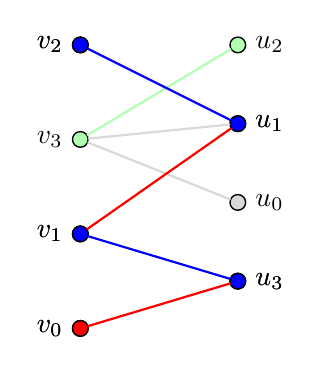
\begin{tikzpicture}
          \GraphInit[vstyle=Classic];
             
          \SetVertexNormal[MinSize=1pt,FillColor=black]
          \Vertex[Math,Lpos=180,x=0,y=0]{v_2};
          \Vertex[Math,Lpos=180,x=0,y=-2.4]{v_1};
          \Vertex[Math,Lpos=180,x=0,y=-3.6]{v_0};
          \Vertex[Math,x=2,y=-1]{u_1};
          \Vertex[Math,x=2,y=-3]{u_3};
          
          \SetVertexNormal[MinSize=1pt,FillColor=blue]
          \Vertex[Math,Lpos=180,x=0,y=0]{v_2};
          \Vertex[Math,Lpos=180,x=0,y=-2.4]{v_1};
          \Vertex[Math,x=2,y=-1]{u_1};
          \Vertex[Math,x=2,y=-3]{u_3};
          
          \SetVertexNormal[MinSize=1pt,FillColor=red]
          \Vertex[Math,Lpos=180,x=0,y=-3.6]{v_0};
          
          \SetVertexNormal[MinSize=1pt,FillColor=green!30]
          \Vertex[Math,Lpos=180,x=0,y=-1.2]{v_3};
          \Vertex[Math,x=2,y=0]{u_2};
          
          \SetVertexNormal[MinSize=1pt,FillColor=gray!30]
          \Vertex[Math,x=2,y=-2]{u_0}
          
          \tikzset{EdgeStyle/.append style={green!30}};
          \Edge(v_3)(u_2);
          
          \tikzset{EdgeStyle/.append style={gray!30}};
          \Edge(v_3)(u_1);
          \Edge(v_3)(u_0);
          
          \tikzset{EdgeStyle/.append style={blue}};
          \Edge(v_2)(u_1);
          \Edge(v_1)(u_3);
          
          \tikzset{EdgeStyle/.append style={red}};
          \Edge(v_1)(u_1);
          \Edge(v_0)(u_3);            
        \end{tikzpicture}
      }
    \end{column}
    \begin{column}{.65\textwidth}
      \onslide<2->{\scriptsize
        Let $R := Ranking(G,\pi,\sigma)$ for a fixed graph $G$, arrival order $\pi$, and ranking $\sigma$.
        \begin{alertblock}{\scriptsize Specification of alternating path}
          \begin{align*}
            zig(x) &=
              \begin{cases}
                x \cons zag(y) & \{x,y\} \in R \\
                [x] & x \text{ unmatched}
              \end{cases} \\\\
            zag(y) &=
              \begin{cases}
                y \cons zag(x') & x' \text{ \alert{matched instead}} \\
                [y] & \text{no other match}
              \end{cases}
          \end{align*}
        \end{alertblock}  
      }
    \end{column}
  \end{columns}
  \onslide<3->
  \begin{itemize}
    \item<3-> \alert{non-recursive} specification of $Ranking(G,\pi,\sigma)$ \textrightarrow interchangeability of $U,V$
    \item<4-> Berge's Lemma~\cite{abdulaziz2019} for repeated application
  \end{itemize}
  \note{
    \begin{itemize}
      \item \emph{non-recursive} specification of matching on $G$ with arrival order $\pi$,
          and ranking $\sigma$
      \item gives interchangeability of offline and online vertices
      \item symmetry \textrightarrow{} $zig$-$zag$ also works for removing online vertex
      \item full specification of path with mutually recursive functions \emph{zig} and \emph{zag}
      \item Berge's Lemma formalized by Abdulaziz~\cite{abdulaziz2019}
      \item Berge's Lemma not required for Lemma 2, but for consequence
    \end{itemize}
  }
\end{frame}

%\begin{frame}
%  \frametitle{Remaining combinatorics}
%\end{frame}

\section{Randomization}
\begin{frame}
  \frametitle{Randomization}
  \begin{itemize}[<+->]
    \item rephrase everything as \emph{\_ pmf} (probability mass function)
    \item finite probability spaces over permutations \textrightarrow{} lots of sums
  \end{itemize}
  \onslide<+->
  \begin{alertblock}{Switching probability spaces}
    \begin{enumerate}[<+->]
      \item choosing a random permutation \textbf{vs.}
      
      \item choosing a random permutation, a random vertex, and putting that vertex at index $t$
    \end{enumerate}
    \onslide<+->
    For $t = 1$ and $V = \{1,2,3\}$:
    \begin{align*}
      \mathbb{P}_1\Big(\big\{[3,2,1]\big\}\Big) &= \frac{1}{3!} \\
      \mathbb{P}_2\Big(\big\{[3,2,1]\big\}\Big) &= \mathbb{P}_1\Big(\big\{[2,3,1], [3,1,2], [3,2,1]\big\}\Big) 
        \cdot \mathbb{P}_V\big(\{2\}\big) \\
        &= \frac{3}{3!} \cdot \frac{1}{3} = \frac{1}{3!}
    \end{align*}
  \end{alertblock}
\end{frame}

\begin{frame}
  \frametitle{References}
  
  \nocite{github-repo}
  \bibliographystyle{alpha}
  \bibliography{../document/root}
\end{frame}

\end{document}

